\chapter{Iteracion 7}
\section{Objetivos de iteración}
\begin{itemize}
 \item Finalizar cliente de GameRegistry para vertx.
 \item Máquina virtual en producción.
 \item Test sobre \emph{Promises}.
\end{itemize}

 
\section{Finalizar cliente de GameRegistry para vert.x}
El cliente asíncrono para el servidor GameRegistry en Java 
es funcional. En el diseño de la API se ha tenido en
cuenta los siguientes factores:

\begin{itemize}
 \item API con estilo fluído. Debería resultar razonablemente 
       familiar para usuarios de otros objetos Vert.x como 
       \texttt{HttpClient} o \texttt{DnsClient}.
 \item Sin dependencias adicionales. Utilizar el cliente
       no debe obligar al usuario a utilizar más dependencias.
       Esto es lo que ha motivado la elección del lenguaje
       (\emph{Java}) y la ausencia en el diseño de 
       \emph{Lambdas} (obligaría a usar \emph{Java 8})
       o \emph{Promises}.
 \item Simpleza de uso. El cliente siempre devolverá 
       tras una petición y de forma asíncrona un objeto
       \emph{GameRegistryResponse} que contendrá la información
       del resultado, sea un error (con un código de error
       y el \emph{Throwable} causante del error incluído)
       o una colección de sesiones de juego. Sólo requiere,
       por tanto, un manejador (\emph{Handler}) por petición
       y es sencillo detectar el resultado de la petición
       con tan solo comprobar el código de resultado.
 \item Hemos procurado que sea capaz de detectar e informar
       de los errores a través de un código de resultado.
\end{itemize}

Los parámetros de filtrado para peticiones GET a la colección
de sesiones de juego siguen sin especificar y por tanto aún
no están implementados.


\section{Máquina virtual en producción}

El servidor esta funcionando en la plataforma \emph{Azure} sobre
una máquina virtual con el siguiente registro DNS:

\textbf{\texttt{gameregistry.cloudapp.net}}

Nuestro servidor escucha peticiones en el puerto \textbf{8080}.
Para acceder a la documentación de \emph{Swagger} se puede utilizar
la siguiente dirección:

\texttt{http://gameregistry.cloudapp.net:8080/doc/}

La API vive en la siguiente dirección:

\texttt{http://gameregistry.cloudapp.net:8080/api/v1}


\subsection{La máquina virtual}
El sistema de despliegue en estos momentos requiere intervención
manual. Los pasos han sido automatizados en gran medida a través
de \emph{scripts Bash} pero sigue siendo necesario identificarse
en la máquina a través de \emph{ssh} y ejecutar el proceso de
despliegue, dividido en 2 o 3 pasos fundamentales (con sus 
correspondientes \emph{scripts}):

\begin{itemize}
 \item Construcción del contenedor \emph{Docker} del servidor.
 \item Si no esta previamente funcionando, lanzar el contenedor 
       \emph{Docker} de \emph{MongoDB}.
 \item Lanzar el contenedor recién construido del servidor.
\end{itemize}


\section{Test sobre \emph{Promises}}
\subsection{Motivación}
En una sesión de clase el profesor nos indicó que debíamos \emph{demostrar}
que el uso de \emph{Promises} en nuestro servidor no bloqueaba el hilo principal
de \emph{Vert.x}. Dado que es una tarea encargada a nuestro
grupo de forma particular vamos a entrar en más detalle del normal en 
la cuestión.

En nuestro servidor utilizamos \emph{Promises} para hacer más legible y sencilla
la programación asíncrona de algunos de los servicios internos (como el servicio
de autenticación que debe validar con el \emph{LoginServer} los pares 
usuario-token de las peticiones realizadas a nuestro servidor). En concreto utilizamos
una implementación para \emph{Groovy}:

\texttt{com.darylteo.vertx:vertx-promises-groovy:1.2.1}

Dicha biblioteca establece en su \texttt{Readme} la siguiente información:

\say{Esta biblioteca implementa la mayor parte de la especificación 
\emph{Promises/A+}. Esta basado en \emph{Q} para \emph{Node.js}, que añade
facilidades adicionales como \texttt{reject} y \texttt{finally}. Finalmente,
esta construida utilizando la biblioteca \emph{RxJava}.}

También menciona la siguiente información:

\say{Esta biblioteca no se parece a otras implementaciones similares basadas
en lenguaje (como \emph{Futures} o \emph{GroovyPromise} en tanto a que
esta completamente libre de bloqueos. Esta diseñada para trabajar con
plataformas que hacen uso intensivo de \emph{callbacks} asíncronos. Es más,
tiene varias clases adicionales que intentan mejorar la seguridad de tipos
del uso basado en \emph{Java} a la vez que minimiza el exceso de \emph{verbosidad}
a través de la inferencia de \emph{generics}.

Por tanto es de esperar que seamos capaces de demostrarlo con un test razonablemente
simple.}

\subsection{El test}
La secuencia del test es la siguiente:

\begin{itemize}
 \item Lanzar desde el test una petición con un \emph{path} específico al servidor.
 \item El servidor, en respuesta a esta petición al \emph{path} específico,
       debe utilizar un \emph{Timer} de \emph{Vert.x} para retrasar su respuesta
       artificialmente un cierto tiempo (20 segundos). Para que el test
       demuestre que \emph{Promises no bloquea} el \emph{Timer} debe iniciarse
       desde dentro de un método que devuelve una \emph{promesa} que sólo será
       cumplida desde el código invocado por el \emph{Timer} al terminar la
       espera.
 \item Un cierto tiempo después de la primera petición el test debe lanzar una
       segunda petición a un \emph{path} del servidor con comportamiento normal
       de forma que este responda antes de que el tiempo de espera artificial
       de la primera petición se cumpla.
 \item Finalmente, el test debe recibir la respuesta a la segunda petición y
       al cabo de 20 segundos de lanzar la primera petición debe recibir la respuesta
       a esta.
\end{itemize}

\subsubsection{Implementación}

En el lado del servidor el código de inicialización del \emph{RouteMatcher} añade
de forma opcional (según el contenido de \emph{conf.json}) una ruta adicional 
con un manejador simple que llama a un nuevo servicio interno llamado
\emph{DebugPromiseService}, que a través de una \emph{promesa} devuelve una
cadena de texto que se utilizará en la respuesta. Más adelante en esta iteración
hay un diagrama de clases actualizado que muestra la estructura general del mismo.

A continuación se muestra el código pertinente del servicio (\emph{Groovy}):

\begin{verbatim}
 Promise<String> doSomething(HttpServerRequest request) {
   final Promise<String> p = new Promise()

   vertx.setTimer(wait_time * 1000, { time ->
     p.fulfill("<html><body>Waited " 
               + wait_time 
               + " seconds to give this answer.</body></html>")
   })

   return p;
 }
\end{verbatim}

El test tiene la siguiente implementación:

\begin{verbatim}
 def testDebugPromiseIsNotBlocking() {
   HttpClient client = vertx.createHttpClient().setPort(8080)
   HttpClient client2 = vertx.createHttpClient().setPort(8080)
   String path = "/debug_promise"
   List<Integer> order = []

   // This gets the first request going
   container.logger.info("#1: Launching first request!")
   order.add(1)

   client.getNow(path, { response ->
     // This code will execute around 20 secs after the 
     // getNow call was performed
     container.logger.info("#4: First request answered.")
     order.add(4)

     assertEquals([1,2,3,4], order)
     testComplete()
   })

   // Wait for 2 seconds
   vertx.setTimer(2 * 1000, {long time ->
     // And then do another request that should end 
     // before the first one.
     container.logger.info("#2: Launching second request!")
     order.add(2)

     client2.getNow("/doc", { response ->
       container.logger.info("#3: Second request answered.")
       order.add(3)
     })
   })
  }
\end{verbatim}

Cabe destacar que la implementación de \texttt{HttpClient} no es capaz de realizar
dos peticiones simultaneas al mismo host en el mismo \emph{verticle}. Resultaba confuso 
porque los resultados del test parecían sugerir que efectivamente el servidor estaba 
bloqueando tras la primera petición pero realmente era el cliente Http el problema. 
Con dos instancias del cliente Http el test pasa sin problemas.


\section{Diagrama UML actualizado}

Se incluyen diagramas UML tanto del servidor como del cliente en su estado actual.

\begin{figure}[h]
 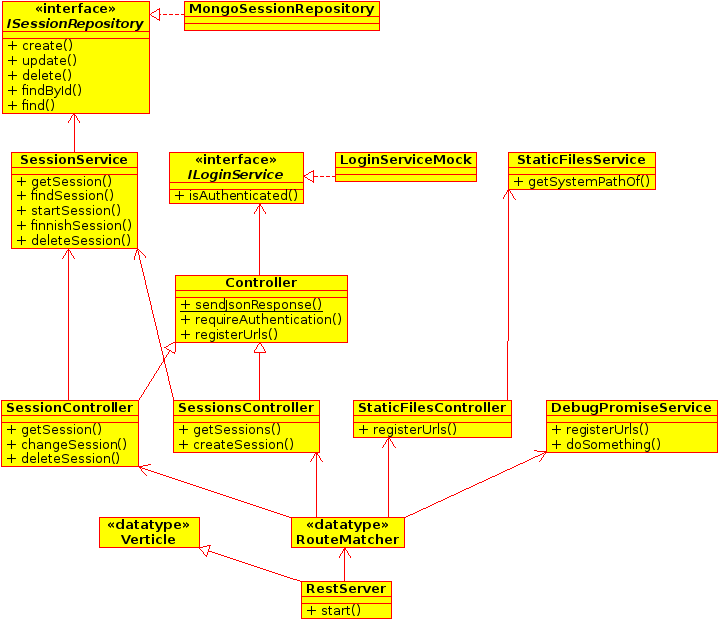
\includegraphics[scale=0.8]{diagrams/class_diagram_iter7.png}
 \caption{Diagrama de clases (iteración 7)}
 \label{fig:clases}
\end{figure} 

\begin{figure}[h]
 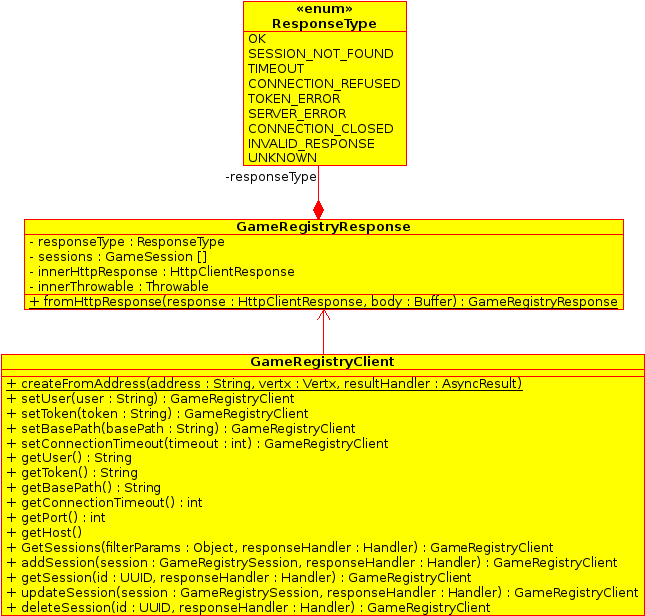
\includegraphics[scale=0.8]{diagrams/class_diagram_client_iter7.png}
 \caption{Diagrama de clases del cliente (iteración 7)}
 \label{fig:clases}
\end{figure} 
